\newpage\setcounter{dang}{0}
\section{PHƯƠNG TRÌNH ĐƯỜNG THẲNG}
\subsection{Tóm tắt lí thuyết}
\subsubsection{Phương trình tổng quát của đường thẳng}
\begin{dn}
	Vectơ $\vec{n}$ khác $\vec{0}$ được gọi là vectơ pháp tuyến của đường thẳng $\Delta$ nếu giá của nó vuông góc với $\Delta$.
\end{dn}
\begin{nx}
	\begin{itemize}
		\item Nếu $\vec{n}$ là vectơ pháp tuyến của đường thẳng $\Delta$ thì $k\vec{n}$ ($k \ne 0$) cũng là vectơ pháp tuyến của $\Delta$.
		\item Đường thẳng hoàn toàn xác định nếu biết một điểm và một vectơ pháp tuyến của nó.
	\end{itemize}
\end{nx}

\begin{vd}
	Trong mặt phẳng toạ độ, cho tam giác có ba đỉnh là $A(3;1)$, $B(4;0)$, $C(5;3)$. Hãy chỉ ra  một vectơ pháp tuyến của đường trung trực của đoạn thẳng $AB$ và một vectơ pháp tuyến của đường cao kẻ từ $A$ của tam giác $ABC$.
	\loigiai{
		Đường trung trực của đoạn $AB$ vuông góc với $AB$ nên có một vectơ pháp tuyến là $\vec{AB}(1;-1)$.
		Đường cao kẻ từ kẻ từ $A$ của tam giác $ABC$ vuông góc với $BC$ nên có một  vectơ pháp tuyến là $\vec{BC}(1;3)$.
	}
\end{vd}

\begin{nx}
	Trong mặt phẳng toạ độ, mọi đường thẳng đều có phương trình tổng quát dạng $ax+by+c=0$, với $a$ và  $b$ không đồng thời bằng $0$. Ngược lại, mỗi phương trình dạng $ax+by+c=0$,  với $a$ và  $b$ không đồng thời bằng $0$, đều là phương trình của một đường thẳng, nhận $\vec{n}(a;b)$ là một vectơ pháp tuyến.
\end{nx}
\begin{vd}
	Trong mặt phẳng toạ độ, lập phương trình tổng quát của đường thẳng $\Delta$ đi qua điểm $A(2;1)$ và nhận $\vec{n}(3;4)$ là một vectơ pháp tuyến.
	\loigiai{
		Đường thẳng $\Delta$ có phương trình là $3(x-2)+4(y-1)=0$ hay $3x+4y-10=0$.
	}
\end{vd}

\begin{vd}
	Trong mặt phẳng toạ độ, cho tam giác có ba đỉnh $A(-1;5)$, $B(2;3)$, $C(6;1)$. Lập phương trình tổng quát của đường cao kẻ từ $A$ của tam giác $ABC$.
	\loigiai{Ta có $\vec{BC}(4;-2)$.\\
		Đường cao kẻ từ kẻ từ $A$ của tam giác $ABC$ vuông góc với $BC$ nên có một  vectơ pháp tuyến là $\vec{n}(2;-1)$.\\
		Đường thẳng $\Delta$ có phương trình là $2(x+1)-(y-5)=0$ hay $2x-y+7=0$.
	}
\end{vd}

\begin{vd}
	Trong mặt phẳng toạ độ, lập phương trình tổng quát của đường thẳng $\Delta$ đi qua điểm $A(0;b)$ và có vectơ pháp tuyến  $\vec{n}(a;-1)$ với $a$, $b$ là các số cho trước. Hãy chỉ ra mối liên hệ giữa đường thẳng $\Delta$ với đồ thị của hàm số $y=ax+b$.
	\loigiai{
		Đường thẳng $\Delta$ có phương trình là $a(x-0)-1(y-b)=0$ hay $ax-y+b=0$.\\
		Đường thẳng $\Delta$ là tập hợp những điểm $M(x;y)$ thoả mãn $ax-y+b=0$, hay là $y=ax+b$.\\
		Do đó, đường thẳng $\Delta: ax-y+b=0$ chính là đồ thị hàm số $y=ax+b$.
	}
\end{vd}

\begin{vd}
	Hãy chỉ ra một vectơ pháp tuyến của đường thẳng $\Delta \colon y=3x+4$.
	\loigiai{
		Đường thẳng $\Delta$ có một vectơ pháp tuyến là $\vec{n}(3;-1)$.
	}
\end{vd}
\begin{nx}
	Trong mặt phẳng toạ độ, cho đường thẳng $ \Delta \colon ax+by+c=0$.
	\begin{itemize}
		\item Nếu $b=0$ thì phương trình có thể đưa về dạng $x=m$ (với $m=-\dfrac{c}{a}$) và $\Delta$ vuông góc với $Ox$.
		\item Nếu $b \ne 0$ thì phương trình có thể đưa về dạng $y=nx+p$ (với $n=-\dfrac{a}{b}$, $m=-\dfrac{c}{b}$).
	\end{itemize}
\end{nx}

\subsubsection{Phương trình tham số của đường thẳng}
\begin{dn}
	Vectơ $\vec{u}$ khác $\vec{0}$ được gọi là vectơ chỉ phương  của đường thẳng $\Delta$ nếu giá của nó song song hoặc trùng  với $\Delta$.
\end{dn}
\begin{nx}
	\begin{itemize}
		\item Nếu $\vec{u}$ là vectơ chỉ phương  của đường thẳng $\Delta$ thì $k\vec{u}$ ($k \ne 0$) cũng là vectơ chỉ phương của $\Delta$.
		\item Đường thẳng hoàn toàn xác định nếu biết một điểm và một vectơ chỉ phương của nó.
		\item Vectơ $\vec{n}(a;b)$ vuông góc với các vectơ $\vec{u}(-b;a)$ và $\vec{v}(b;-a)$ nên nếu $\vec{n}$ là vectơ pháp tuyến của đường thẳng $\Delta$ thì $\vec{u}$, $\vec{v}$ là hai vectơ chỉ phương của đường thẳng đó và ngược lại.
	\end{itemize}
\end{nx}

\begin{vd}
	Trong mặt phẳng toạ độ, cho  $A(3;2)$, $B(1;-4)$. Hãy chỉ ra  hai  vectơ chỉ phương  của đường  thẳng $AB$.
	\loigiai{
		Đường  thẳng $AB$ nhận  $\vec{AB}(-2;-6)$ là một vectơ chỉ phương.\\
		Lấy  $\vec{u}=-\dfrac{1}{2}\vec{AB}=(1;3)$, khi đó  $\vec{u}$ cũng là một vectơ chỉ phương của đường thẳng $AB$.
	}
\end{vd}

\begin{vd}
	Hãy chỉ ra một vectơ  chỉ phương  của đường thẳng $\Delta \colon 2x-y+1=0$.
	\loigiai{
		Đường thẳng $\Delta$ có một vectơ chỉ phương là $\vec{n}(1;2)$.
	}
\end{vd}
\begin{dn}
	Cho đường thẳng $\Delta$ đi qua điểm $A(x_0;y_0)$ và có vectơ chỉ phươn g$\vec{u}(a;b)$. Khi đó điểm $M(x;y)$  thuộc  đường thẳng $\Delta$ khi và chỉ khi tôn tại số thực $t$ sao cho $\vec{AM}=t\vec{u}$, hay 
	\[\heva{&x=x_0+at\\&y=y_0+bt.} \quad \quad (2)\]
	Hệ $(2)$ được gọi là phương trình tham số của đường thẳng $\Delta$ ($t$ là tham số).
\end{dn}

\begin{vd}
	Lập phương trình tham số của đường thẳng $\Delta$ đi qua $M(2;-3)$ và có  vectơ  chỉ phương $\vec{u}(4;-1)$.
	\loigiai{
		Phương trình tham số của đường thẳng $\Delta$  là $\heva{&x=2+4t\\&y=-3-t.}$
	}
\end{vd}

\begin{vd}
	Lập phương trình tham số của đường thẳng $\Delta$ đi qua $M(-1;2)$ và song song với đường thẳng $d \colon 3x-4y-1=0$.
	\loigiai{ Đường thẳng $\Delta$  song song với đường thẳng $d \colon 3x-4y-1=0$ nên có một vectơ chỉ phương là  $\vec{u}(4;3)$.\\
		Phương trình tham số của đường thẳng $\Delta$  là $\heva{&x=-1+4t\\&y=2+3t.}$
	}
\end{vd}

\begin{vd}
	Lập phương trình tham số của đường thẳng $\Delta$ đi qua hai điểm  $A(2;3)$ và $B(1;5)$.
	\loigiai{ Đường thẳng $\Delta$  đi qua hai điểm  $A(2;3)$ và $B(1;5)$  nên có một vectơ chỉ phương là  $\vec{u}=\vec{AB}=(-1;2)$.\\
		Phương trình tham số của đường thẳng $\Delta$  là $\heva{&x=2-t\\&y=3+2t.}$
	}
\end{vd}

\begin{vd}
	Lập phương trình tham số và phương trình tổng quát của đường thẳng $\Delta$ đi qua hai điểm  phân biệt  $A(x_1;y_1)$ và $B(x_2;y_2)$ cho trước.
	\loigiai{ Đường thẳng $\Delta$  đi qua hai điểm $A(x_1;y_1)$ và $B(x_2;y_2)$  nên có một vectơ chỉ phương là  $\vec{u}=\vec{AB}=(x_2-x_1;y_2-y_1)$.\\
		Phương trình tham số của đường thẳng $\Delta$  là $\heva{&x=x_1+(x_2-x_1)t\\&y=y_1+(x_2-x_1)t.}$\\
		Ta có một vectơ pháp tuyến của đường thẳng $\Delta$ là $\vec{n}=(y_1-y_2;x_2-x_1)$.\\ Phương trình tổng quát của $\Delta$ là $((y_1-y_2)(x-x_1)+(x_2-x_1)(y-y_1)=0$
	}
\end{vd}

\subsection{Các dạng toán thường gặp}
\begin{dang}{Xác định các yếu tố của đường thẳng}
	\begin{itemize}
		\item Đường thẳng $\Delta: \heva{&x=x_0+at\\&y=y_0+bt}\,\,\,t\in\mathbb{R}$ có điểm đi qua là $M\left(x_0;y_0\right)$ và có vectơ chỉ phương là $\vec{u}=\left(a;b\right)$.
		\item Đường thẳng $\Delta: ax+by+c=0$ có vectơ pháp tuyến là $\vec{n}=\left(a;b\right)$.
	\end{itemize}
	
\end{dang}

\begin{vd}
	Hãy chỉ ra một vectơ pháp tuyến của đường thẳng $\Delta\colon y=3x+4$.
	\loigiai{
		$\Delta\colon y=3x+4\Leftrightarrow 3x-y+4=0$.\\
		Vectơ pháp tuyến của đường thẳng $\Delta$ là $\overrightarrow{n_\Delta}=(3;\,-1)$.}
\end{vd}
\begin{vd}
	Trong mặt phẳng tọa độ, cho $A(3;\,2)$, $B(1;\,-4)$. Hãy chỉ ra vectơ chỉ phương của đường thẳng $AB$.
	\loigiai{
		Đường thẳng $AB$ nhận $\overrightarrow{AB}=(-2;\,-6)$ là một vectơ chỉ phương.\\
		Lấy $\overrightarrow{u}=-\dfrac{1}{2}\overrightarrow{AB}=(1;\,3)$, khi đó $\overrightarrow{u}$ cũng là một vectơ chỉ phương của đường thẳng $\overrightarrow{AB}$.
	}
\end{vd}
\begin{vd}
	Hãy chỉ ra một vectơ chỉ phương của đường thẳng $\Delta\colon 2x-y+1=0$
	
	\loigiai{
		$\Delta\colon y=3x+4\Leftrightarrow 3x-y+4=0$.\\
		Vectơ pháp tuyến của đường thẳng $\Delta$ là $\overrightarrow{n_\Delta}=(2;\,-1)$.\\
		Khi đó vectơ chỉ phương của đường thẳng $\Delta$ là $\overrightarrow{n_\Delta}=(1;\,2)$.}
\end{vd}

\begin{vd}
	Trong mặt phẳng tọa độ, cho tam giác có ba đỉnh là $A(3;\,1)$, $B(4;\,0)$, $C(5;\,3)$. Hãy chỉ ra một vectơ pháp tuyến của đường trung trực của đoạn thẳng $AB$ và một vectơ pháp tuyến của đường cao kẻ từ $A$ của tam giác $ABC$.
	\loigiai{
		Đường trung trực của đoạn thẳng $AB$ vuông góc với $AB$ nên có vectơ pháp tuyến $\overrightarrow{AB}=(1;\,-1)$.\\
		Đường cao kẻ từ $A$ của tam giác $ABC$ vuông góc với $BC$ nên có vectơ pháp tuyến $\overrightarrow{BC}=(1;\,3)$.
	}
\end{vd}

\begin{dang}{Viết phương trình đường thẳng}
	Các dạng đường thẳng:
	\begin{itemize}
		\item Đường thẳng $\Delta: \heva{& \text{ có vectơ pháp tuyến là } \vec{n}=\left(a;b\right)\\& \text{ đi qua điểm } M\left(x_0;y_0\right)}$ có phương trình tổng quát là $$\Delta: a\left(x-x_0\right)+b\left(y-y_0\right)=0.$$ 
		\item Đường thẳng $\Delta: \heva{& \text{ có vectơ chỉ phương là } \vec{v}=\left(a;b\right)\\& \text{ đi qua điểm } M\left(x_0;y_0\right)}$ có phương trình tham số là $$\Delta: \heva{&x=x_0+at\\&y=y_0+bt}\,\,\,(t\in \mathbb{R}).$$ 
	\end{itemize}
	\begin{note}
		\textbf{Lưu ý:}
		\begin{itemize}
			\item Đường thẳng $\Delta$ có vectơ pháp tuyến $\vec{n}=(a;b)$ thì có vectơ chỉ phương $\vec{u}=(b;-a)$ hoặc $\vec{u}=(-b;a)$.
			\item Đường thẳng $\Delta$ có hệ số góc $k$ thì có vectơ chỉ phương là $\vec{u}=(1;k)$.
		\end{itemize}
	\end{note}
	
\end{dang}


\begin{vd}
	Viết phương trình tổng quát của đường thẳng $\Delta_1$ đi qua $A(0;1)$ và có vectơ pháp tuyến là $\vec{n}=(3;4)$.
	\loigiai{
		Phương trình tổng quát của đường thẳng $\Delta_1 : \heva{& \text{ có vectơ pháp tuyến là } \vec{n}=\left(3;4\right)\\& \text{ đi qua điểm } A\left(0;1\right)}$ là 
		$$3(x-0)+4(y-1)=0\Leftrightarrow 3x+4y-4=0.$$
	}
\end{vd}

\begin{vd}
	Viết phương trình tổng quát của đường thẳng $\Delta_2$ đi qua $B(2;-3)$ và có vectơ chỉ phương là  $\vec{u}=(1;-2)$.
	\loigiai{
		Phương trình tổng quát của đường thẳng $\Delta_2 :\heva{& \text{ có vectơ chỉ phương là } \vec{v}=\left(1;-2\right)\\& \text{ đi qua điểm } B\left(2;-3\right)}$ là 
		$$\heva{&x=2+1t\\&y=-3-2t}\,\,\,(t\in \mathbb{R}).$$
	}
\end{vd}


\begin{vd}
	Viết phương trình tham số và tổng quát của đường thẳng $AB$ biết $A(0;1)$, $B(2;-3)$.
	\loigiai{
		Đường thẳng $AB$ có vectơ chỉ phương là $\vec{AB}=(2;-4)$, có vectơ pháp tuyến là $\vec{n}_{AB}=(4;2)$.\\
		Phương trình tham số của đường thẳng $AB$ là 
		$$\heva{&x=2t\\&y=1-4t}\,\,\,(t\in \mathbb{R}).$$
		Phương trình tổng quát của đường thẳng $AB$ là $$4(x-0)+2(y-1)=0\Leftrightarrow 4x+2y-2=0.$$
	}
\end{vd}

\begin{vd}
	Viết phương trình tham số của đường thẳng $\Delta$ đi qua $M(-1;3)$ biết hệ số góc của đường thẳng là $k=2$.
	\loigiai{
		Đường thẳng $\Delta$ biết hệ số góc của đường thẳng là $k=2$ suy ra $\Delta$ có vectơ chỉ phương là $\vec{u}=(1;2)$.\\
		Phương trình tham số của $\Delta$ là
		$$\heva{&x=-1+t\\&3+2t}\,\,\,(t\in\mathbb{R}).$$
	}
\end{vd}

\begin{vd}
	Trong mặt phẳng tọa độ, cho tam giác $ABC$ có ba đỉnh $A(-2;5)$, $B(2;1)$, $C(5;2)$. Lập phương trình tổng quát của đường cao kẻ từ $A$ của tam giác $ABC$.
	\loigiai{
		Gọi $AH$ là đường cao kẻ từ $A$ của tam giác $ABC$, khi đó $AH$ vuông góc $BC$.\\
		Suy ra $AH$ có vectơ pháp tuyến là $\vec{BC}=(3;1)$.\\
		Phương trình đường cao $AH$ là
		$$3(x+2)+1(y-5)=0\Leftrightarrow 3x+y+1=0.$$
	}
\end{vd}


\begin{dang}{Bài toán thực tế}
\end{dang}
\begin{vd}
	Đường thẳng $\Delta$ ở hình bên dưới biểu thị tổng chi phí lắp đặt và tiền cước sử dụng dịch vụ Internet (đơn vị: trăm nghìn đồng) theo thời gian của một gia đình (đơn vị: tháng).\\
	\begin{enumerate}
		\item Viết phương trình của đường thẳng $\Delta$.
		\item Cho biết giao điểm của đường thẳng $\Delta$ với trục tung trong tình huống này có ý nghĩa gì.
		\item Tính tổng chi phí lắp đặt và sử dụng Internet trong $12$ tháng đầu tiên.
	\end{enumerate}
	\begin{center}
		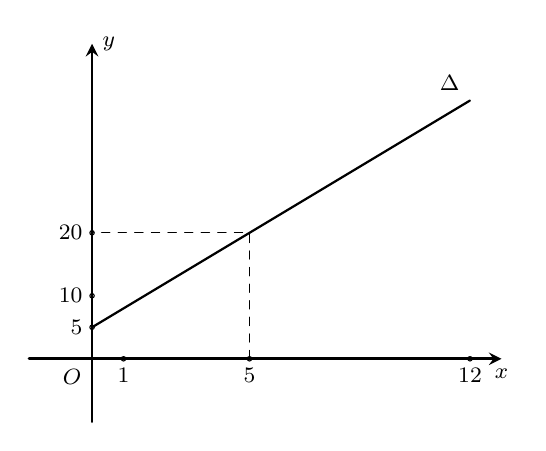
\begin{tikzpicture}[scale=0.8, font=\footnotesize, line join=round, line cap=round, >=stealth]
			\draw[->,line width = 1pt] (-1,0)--(0,0) node[below left]{$O$}--(6.5,0) node[below]{$x$};
			\draw[->,line width =1 pt] (0,-1)--(0,5) node[right]{$y$};
			\draw [thick,domain=0:6,samples=100] 
			plot (\x,{(3/5)*(\x)+1/2}) node [above left] {$\Delta$};
			\draw (0,0.5) node [left] {$5$} circle (1pt);
			\draw (0,1) node [left] {$10$} circle (1pt);		
			\draw (0,2) node [left] {$20$} circle (1pt);
			\draw (0.5,0) node [below] {$1$} circle (1pt);
			\draw (2.5,0) node [below] {$5$} circle (1pt);
			\draw (6,0) node [below] {$12$} circle (1pt);
			\draw [dashed] (2.5,0)--(2.5,2)--(0,2);
		\end{tikzpicture}	
	\end{center}
	\loigiai{
		\begin{enumerate}
			\item Đường thẳng $\Delta$ đi qua hai điểm lần lượt có tọa độ $(0;\,5)$ và $(5;\,20)$ nên $\Delta$ có phương trình là
			$$\dfrac{x-0}{5-0}=\dfrac{y-5}{20-5}\Leftrightarrow\dfrac{x}{5}=\dfrac{y-5}{15}\Leftrightarrow\dfrac{x}{1}=\dfrac{y-5}{3}\Leftrightarrow3x-y+5=0\Leftrightarrow y=3x+5.$$
			\item Giao điểm của đường thẳng $\Delta$ với trục $Oy$ ứng với $x=0$. Thời điểm $x=0$ cho biết mức phí ban đầu lắp đặt để sử dụng Internet. Khi $x=0$ thì $y=5$, vì vậy chi phí lắp đặt ban đầu là $500000$ đồng.
			\item $12$ tháng đầu tiên ứng với $x=12$. Do đó $y=3\cdot12+5=41$.\\
			Vậy tổng chi phí lắp đặt và sử dụng Internet trong $12$ tháng đầu tiên là $4100000$ đồng.
		\end{enumerate}
		
	}
\end{vd}
\begin{vd}
	Để tham gia một phòng tập thể dục, người tập phải trả một khoản phí tham gia ban đầu và phí sử dụng phòng tập. Đường thẳng $\Delta$ ở hình bên dưới biểu thị tổng chi phí (đơn vị: triệu đồng) tham gia một phòng tập thể dục theo thời gian tập của một người (đơn vị: tháng).\\
	\begin{enumerate}
		\item Viết phương trình của đường thẳng $\Delta$.
		\item Cho biết giao điểm của đường thẳng $\Delta$ với trục tung trong tình huống này có ý nghĩa gì.
		\item Tính tổng chi phí mà người đó phải trả khi tham gia phòng tập thể dục với thời gian $12$ tháng.
	\end{enumerate}
	\begin{center}
		\begin{tikzpicture}[scale=0.8, font=\footnotesize, line join=round, line cap=round, >=stealth]
			\draw[->,line width = 1pt] (-1,0)--(0,0) node[below left]{$O$}--(8,0) node[below]{$x$};
			\draw[->,line width =1 pt] (0,-1)--(0,8) node[right]{$y$};
			\draw [thick,domain=0:6,samples=100] 
			plot (\x,{(\x)+3/2}) node [above left] {$\Delta$};
			\draw (0,1) node [left] {$1$} circle (1pt);
			\draw (0,1.5) node [left] {$1{,}5$} circle (1pt);		
			\draw (0,5) node [left] {$5$} circle (1pt);
			\draw (0.5,0) node [below] {$1$} circle (1pt);
			\draw (3.5,0) node [below] {$7$} circle (1pt);
			\draw (6,0) node [below] {$12$} circle (1pt);
			\draw [dashed] (3.5,0)--(3.5,5)--(0,5);
		\end{tikzpicture}	
	\end{center}
	\loigiai{
		\begin{enumerate}
			\item Đường thẳng $\Delta$ đi qua hai điểm lần lượt có tọa độ $(0;\,1{,}5)$ và $(7;\,5)$ nên $\Delta$ có phương trình là
			$$\dfrac{x-0}{7-0}=\dfrac{y-1{,}5}{5-1{,}5}\Leftrightarrow\dfrac{x}{7}=\dfrac{y-1{,}5}{3{,}5}\Leftrightarrow\dfrac{x}{2}=\dfrac{y-1{,}5}{1}\Leftrightarrow y=\dfrac{x}{2}+1{,}5.$$
			\item Giao điểm của đường thẳng $\Delta$ với trục $Oy$ ứng với $x=0$. Thời điểm $x=0$ cho biết mức phí tham gia ban đầu và phí sử dụng phòng tập. Khi $x=0$ thì $y=1{,}5$, vì vậy chi phí tham gia ban đầu và phí sử dụng phòng tập là $1500000$ đồng.
			\item $12$ tháng đầu tiên ứng với $x=12$. Do đó $y=\dfrac{12}{2}+1{,}5=7{,}5$.\\
			Vậy tổng chi phí mà người đó phải trả khi tham gia phòng tập thể dục với thời gian $12$ tháng đầu tiên là $7500000$ đồng.
		\end{enumerate}
		
	}
\end{vd}


\subsection{Bài tập tự luận}
\begin{bt}%[0H3B1-2]
	Trong mặt phẳng $Oxy$, cho $\overrightarrow{n}=(2;1)$, $\overrightarrow{v}=(3;2)$, $A(1;3)$, $B(-2;1)$.
	\begin{enumerate}
		\item Lập phương trình tổng quát của đường thẳng $\Delta_1$ đi qua $A$ và có vectơ pháp tuyến $\overrightarrow{n}$.
		\item Lập phương trình tham số của đường thẳng $\Delta_2$ đi qua $B$ và có vectơ chỉ phương $\overrightarrow{v}$.
		\item Lập phương trình tham số của đường thẳng $AB$.
	\end{enumerate}
	\loigiai{
		\begin{enumerate}
			\item Phương trình tổng quát của $\Delta_1\colon 2\cdot(x-1)+1\cdot(y-3)=0$ hay $\Delta_1\colon 2x+y-5=0$.
			\item Phương trình tham số của $\Delta_2\colon \heva{&x=-2+3t\\&y=1+2t}\quad (t\in\mathbb{R})$.
			\item Ta có $\overrightarrow{AB}=(-3;-2)$ là một vectơ chỉ phương của đường thẳng $AB$.\\
			Phương trình tham số của đường thẳng $AB\colon \heva{&x=1-3s\\&y=3-2s} \quad (s\in\mathbb{R})$.
		\end{enumerate}	
	}
\end{bt}

\begin{bt}%[0H3B1-2]
	Trong mặt phẳng $Oxy$, lập phương trình tổng quát các trục tọa độ.
	\loigiai{
		\begin{enumerate}
			\item Trục $Ox$ có vectơ pháp tuyến là $\overrightarrow{j}=(0;1)$ nên phương trình tổng quát của \linebreak $Ox\colon 0\cdot(x-1)+1\cdot(y-0)=0$ hay $Ox\colon y=0$.
			\item Tương tự, phương trình tổng quát của $Oy\colon x=0$.
		\end{enumerate}
	}
\end{bt}

\begin{bt}%[0H3B1-2]
	Trong mặt phẳng $Oxy$, cho hai đường thẳng $\Delta_1\colon \heva{&x=1+2t\\&y=3+5y}$ và $\Delta_2\colon 2x+3y-5=0$.
	\begin{enumerate}
		\item Lập phương trình tổng quát của $\Delta_1$.
		\item Lập phương trình tham số của $\Delta_2$.
	\end{enumerate}
	\loigiai{
		\begin{enumerate}
			\item Ta có $\Delta_1\colon \heva{&x=1+2t\\&y=3+5y} \Rightarrow 5x-2y+1=0$.\\
			Vậy phương trình tổng quát của $\Delta_1\colon 5x-2y+1=0$.
			\item Chọn $x=1+3s$ suy ra $y=1-2s$.\\
			Vậy phương trình tham số của $\Delta_2\colon \heva{&x=1+3s\\&y=1-2s} \quad (s\in\mathbb{R})$.
		\end{enumerate}
	}
\end{bt}

\begin{bt}%[0H3B1-2]
	Trong mặt phẳng $Oxy$, cho tam giác $ABC$ có $A(1;2)$, $B(3;0)$ và $C(-2;-1)$.
	\begin{enumerate}
		\item Lập phương trình đường cao kẻ từ $A$.
		\item Lập phương trình đường trung tuyến kẻ từ $B$.
	\end{enumerate}
	\loigiai{
		\begin{enumerate}
			\item Gọi $AH$ là đường cao kẻ từ $A$.\\
			Ta có $AH$ nhận $\overrightarrow{n}=-\overrightarrow{BC}=(5;1)$ là vectơ pháp tuyến.\\
			Phương trình tổng quát của đường cao $AH\colon 5\cdot(x-1)+1\cdot(y-2)=0$ hay $AH\colon 5x+y-7=0$.
			\item Ta có $M\left(-\dfrac{1}{2};\dfrac{1}{2}\right)$ là trung điểm của $AC$.\\
			Đường trung tuyến $BM$ nhận $\overrightarrow{u}=-2\overrightarrow{BM}=(7;-1)$ là vectơ chỉ phương.\\
			Phương trình tham số của $BM\colon \heva{&x=3+7t\\&y=-t} \quad (t\in\mathbb{R})$.
		\end{enumerate}
	}
\end{bt}

\begin{bt}%[0H3B1-2]
	Trong mặt phẳng $Oxy$, chứng minh rằng đường thẳng đi qua hai điểm $A(a;0)$, $B(0;b)$ với $ab\ne 0$ có phương trình là $\dfrac{x}{a}+\dfrac{y}{b}=1$. (phương trình đoạn chắn của đường thẳng)
	\loigiai{
		Gọi $\Delta\colon \dfrac{x}{a}+\dfrac{y}{b}=1$.\\
		Ta có $\heva{&\dfrac{a}{a}+\dfrac{0}{b}=1\quad\text{(luôn đúng)}\\&\dfrac{0}{a}+\dfrac{b}{b}=1\quad\text{(luôn đúng)}} \Rightarrow \heva{&A\in\Delta\\&B\in\Delta.}$\\
		Vậy phương trình của $AB\colon \dfrac{x}{a}+\dfrac{y}{b}=1$.
	}
\end{bt}

\begin{bt}%[0H3B1-7]
	Theo Google Maps, sân bay Nội Bài có vĩ độ $21{,}2^\circ$ Bắc, kinh độ $105{,}8^\circ$ Đông, sân bay Đà Nẵng có vĩ độ $16{,}1^\circ$ Bắc, kinh độ $108{,}2^\circ$ Đông. Một máy bay, bay từ sân bay Nội Bài đến sân bay Đà Nẵng. Tại thời điểm $t$ giờ, tính từ lúc xuất phát, máy bay ở vị trí có vĩ độ $x^\circ$ Bắc, kinh độ $y^\circ$ Đông được tính theo công thức $\heva{&x=21{,}2-\dfrac{153}{40}t\\&y=105{,}8+\dfrac{9}{5}t.}$
	\begin{enumerate}
		\item Hỏi chuyến bay từ Nội Bài đến Đà Nẵng mất mấy giờ?
		\item Tại thời điểm $1$ giờ kể từ lúc cất cánh, máy bay đã bay qua vĩ tuyến $17$ ($17^\circ$ Bắc) chưa?
	\end{enumerate}
	\loigiai{
		\begin{enumerate}
			\item Xét $x=16{,}1 \Leftrightarrow 21{,}2-\dfrac{153}{40}t=16{,}1 \Leftrightarrow t=\dfrac{4}{3}$ giờ.
			\item Tại thời điểm $1$ giờ, máy bay ở vĩ độ $x=21{,}2-\dfrac{153}{40}\cdot 1=17{,}37$.\\
			Vậy máy bay chưa bay qua vĩ tuyến $17$ ($17^\circ$ Bắc).
		\end{enumerate}
	}
\end{bt}
\subsection{Bài tập trắc nghiệm}
\Opensolutionfile{ans}[ans]
% Câu 1
\begin{ex}%[0H3Y1-2]
	Đường thẳng đi qua $A\left(-1; 2\right)$, nhận $\overrightarrow{n}=(2;-4)$ làm véctơ pháp tuyến có phương trình là
	\choice
	{$x+2y+4=0$}
	{\True $x-2y+5=0$}
	{$x-2y-4=0$}
	{$x+y+4=0$}
	\loigiai{
		Đường thẳng đi qua $A\left(-1; 2\right)$, nhận $\overrightarrow{n}=(2;-4)$ làm véctơ pháp tuyến có phương trình là
		\[2\left(x+1\right)-4\left(y-2\right)=0\Leftrightarrow x-2y+5=0.\]
	}
\end{ex}
% Câu 2
\begin{ex}%[0H3Y1-2]
	Đường thẳng đi qua điểm $M\left(1;2\right)$ và vuông góc với vec-tơ $\overrightarrow{n}=\left(2;3\right)$ có phương trình chính tắc là
	\choice
	{$\dfrac{x-1}{2}=\dfrac{y-2}{3}$}
	{\True $\dfrac{x-1}{3}=\dfrac{y-2}{-2}$}
	{$\dfrac{x+1}{2}=\dfrac{y+2}{3}$}
	{$\dfrac{x+1}{-3}=\dfrac{y+2}{2}$}
	\loigiai{
		Ta có vec-tơ pháp tuyến của đường thẳng là $\overrightarrow{n}=\left(2;3\right)$, do đó vec-tơ chỉ phương của đường thẳng là $\overrightarrow{u}=\left(3;-2\right)$.\\
		Phương trình chính tắc của đường thẳng đi qua $M\left(1;2\right)$ và có vec-tơ chỉ phương $\overrightarrow{u}=\left(3;-2\right)$ là $\dfrac{x-1}{3}=\dfrac{y-2}{-2}$.}
\end{ex}
% Câu 3
\begin{ex}%[0H3B1-2]
	Cho tam giác $ABC$ có $A(2;0), B(0;3), C(-3;1)$. Đường thẳng qua $B$ và song song với $AC$ có phương trình là
	\choice
	{$x-5y+15=0$}
	{$5x-y+3=0$}
	{$5x+y-3=0$}
	{\True $x+5y-15=0$}
	\loigiai{
		Ta có $\overrightarrow{AC}=(-5;1)$, vậy phương trình đường thẳng cần tìm là $\dfrac{x-0}{-5}=\dfrac{y-3}{1}\Leftrightarrow x+5y-15=0$.}
\end{ex}
% Câu 4
\begin{ex}%[0H3B1-2]
	Viết phương trình đường thẳng qua giao điểm của hai đường thẳng $2x-y+5=0$ và $3x+2y-3=0$ và đi qua điểm $A(-3;-2)$
	\choice
	{\True $5x-2y+11=0$}
	{$2x-5y+11=0$}
	{$5x+2y+11=0$}
	{$x-y-3=0$}
	\loigiai{
		Gọi $B$ là tọa độ giao điểm của 2 đường thẳng.\\
		Tọa độ $B$ thỏa mãn hệ \[\heva{
			& 2x-y+5=0 \\ 
			& 3x+2y-3=0 \\}\Leftrightarrow \heva{
			& 2x-y=-5 \\ 
			& 3x+2y=3 \\}\Leftrightarrow \heva{
			& x=-1 \\ 
			& y=3 \\}\Rightarrow B\left(-1;3\right).\]
		Ta có $\overrightarrow{AB}=\left(2;5\right)$, khi đó $\overrightarrow{n}_{AB}=\left(5;-2\right)$.\\
		Phương trình đường thẳng là $AB\colon 5\left(x+3\right)-2\left(y+2\right)=0\Leftrightarrow 5x-2y+11=0$.}
\end{ex}
% Câu 5
\begin{ex}%[0H3B1-2]
	Cho hai điểm $A(4;-1);B(1;-4)$. Viết phương trình tổng quát đường trung trực của đoạn thẳng $AB$.
	\choice
	{$x-y=0$}
	{$x-y=1$}
	{$x+y=1$}
	{\True $x+y=0$}
	\loigiai{
		$\overrightarrow{AB}=(-3;-3)=-3(1;1)$. Gọi $M$ là trung điểm của $AB$ thì $M\left(\dfrac{5}{2};-\dfrac{5}{2}\right)$.\\
		Đường trung trực của đoạn thẳng $AB$ đi qua $M\left(\dfrac{5}{2};-\dfrac{5}{2}\right)$ và nhận $\overrightarrow{n}=(1;1)$ làm một vec-tơ pháp tuyến nên có phương trình tổng quát  \[\left(x-\dfrac{5}{2}\right)+\left(y+\dfrac{5}{2}\right)=0\Leftrightarrow x+y=0.\]}
\end{ex}
% Câu 6
\begin{ex}%[0H3Y1-2]
	Cho đường thẳng $\Delta\colon y=-\dfrac{3}{2}x+1$. Vec-tơ nào sau đây không là vec-tơ chỉ phương của $\Delta $?
	\choice
	{\True $\left(-3;2\right)$}
	{$\left(2;3\right)$}
	{$\left(1;-\dfrac{3}{2}\right)$}
	{$\left(-2;3\right)$}
	\loigiai{
		Đường thẳng $\Delta\colon y=-\dfrac{3}{2}x+1$ có hệ số góc $k=-\dfrac{3}{2}=\dfrac{u_2}{u_1}$, với $\overrightarrow{u}=\left(u_1;u_2\right)$ là VTCP của $\Delta $.\\
		Loại trừ các VTCP của $\Delta $ khi chọn $u_1=\left\{1;2;-2\right\}$.\\
		Vậy vec-tơ không là VTCP cần tìm là $\left(-3;2\right)$.}
\end{ex}
% Câu 7
\begin{ex}%[0H3B1-2]
	Viết phương trình tham số của đường thẳng đi qua điểm $O\left(0;0\right)$ và song song với đường thẳng $\Delta \colon 3x-4y+1$.
	\choice
	{$\heva{
			& x=-3t \\ 
			& y=4t \\}$}
	{$\heva{
			& x=3t \\ 
			& y=-4t \\}$}
	{\True $\heva{
			& x=4t \\ 
			& y=3t \\}$}
	{$\heva{
			& x=4t \\ 
			& y=1+3t \\}$}
	\loigiai{
		Thay tọa độ điểm $O$ vào phương trình đường thẳng $\Delta $ thấy không thỏa mãn.\\
		Do hai đường thẳng song song nên đường thẳng cần tìm nhận $\overrightarrow{u}\left(4;3\right)$ làm vec-tơ chỉ phương.\\
		Phương trình tham số của đường thẳng cần tìm $\heva{
			& x=4t \\ 
			& y=3t. \\}$
	}
\end{ex}
% Câu 8
\begin{ex}%[0H3B1-2]
	Cho tam giác $ABC$ có tọa độ các đỉnh là $A\left(1;2\right)$, $B\left(3;1\right)$, và $C\left(5;4\right)$. Phương trình nào sau đây là phương trình đường cao của tam giác vẽ từ $A$?
	\choice
	{$5x-6y+7=0$}
	{$3x-2y+5=0$}
	{\True $2x+3y-8=0$}
	{$3x-2y-5=0$}
	\loigiai{
		Đường cao vẽ từ $A$ đi qua điểm $A\left(1;2\right)$ và nhận $\overrightarrow{BC}=\left(2;3\right)$ làm vectơ pháp tuyến có phương trình $2x+3y-8=0$.}
\end{ex}
% Câu 9
\begin{ex}%[0H3Y1-2]
	Cho đường thẳng $\Delta \colon \heva{
		& x=15 \\ 
		& y=6+7t \\}$. Viết phương trình tổng quát của $\Delta $.
	\choice
	{$x+15=0$}
	{$6x-15y=0$}
	{\True $x-15=0$}
	{$x-y-9=0$}
	\loigiai{
		Đường thẳng có vtcp $\overrightarrow{u}=\left(0;7\right)$ nên có vtpt $\overrightarrow{n}=\left(1;0\right)$.\\
		Đường thẳng $\Delta $ đi qua điểm $\left(15;6\right)$ nên có phương trình tổng quát là $x-15=0$.}
\end{ex}
\Closesolutionfile{ans}